\documentclass{article}
\usepackage{url}
\usepackage{listings}
\usepackage{float}
\usepackage{graphicx}


\title{\vspace{-4cm}COMP423 Assignment Report: Text Classification}
\date{\today}
\author{Brandon Scott-Hill - 300362945}

\begin{document}

\maketitle

\section{Description}
The baseline system used a bag of words model and movie review dataset to perform text classification task to tell if a movie review is a good review or a bad review. The baseline system uses python with the packages Keras, Tensorflow and NLTK. Keras and Tensorflow are used to create and evaluate the bag of words model and NLTK or Natural language Toolkit to get a set of stop words used for filtering stops words in the data. The baseline system works by 3 Steps. First by loading a vocab file representing the set of known words to the model. Second, the baseline imports the different classes from the data which goes through a cleaning process which returns training data, training labels, testing data, and testing label. Third, the data is used to create and then evaluates the model by using Keras with Keras’ the tokeniser system to convert text data to machine-readable format and Keras’ Sequential model system to create, fit and evaluate the bag of words model.

\section{Instructions} 

To apply a new dataset first some cleaning of the data must occur this includes the following: Removing all punctuation, making all words lower case, removing all word with symbols, removing words with one letter, removing words longer 16 characters, and removing all stops words.\\
\\
Next you need to create vocab text file with store every word in the dataset after the data cleaning like so:

\begin{lstlisting}
create_vocab_file(["dirPath1", "dirPath2"])
\end{lstlisting}

\noindent 
Once the vocab file has being created you must load vocab file and load the different classes of the data set then finally passing the classes to the model like so:

\begin{lstlisting}
vocab = load_vocab_file("vocab.txt")
class1 = get_class("dirPath1", "dirPathTest1", 0)
class2 = get_class("dirPath2", "dirPathTest2", 1)
class3 = get_class("dirPath3", "dirPathTest3", 2)
model([class1, class2, class3])
\end{lstlisting}

\noindent
Fortunately, there is python file with a pre generated vocab file already set up with a new dataset called 20 newsgroups cleaned at runtime, to run the already set up python file with the new dataset perform the following commands at local directory of the code base:

\begin{lstlisting}
source env/Scripts/activate or source env/bin/activate
py basline-newdata.py
\end{lstlisting}

\noindent
If you don't already have the virtual environment setup as required run the following commands at local directory of the code base: 
\begin{lstlisting}
py -m pip install --user virtualenv
py -m venv env
source env/Scripts/activate or source env/bin/activate
pip install keras
pip install tensorflow
pip install nltk
\end{lstlisting}


\section{Modification}

The modification was switching and testing for better text representation method for the dataset. The tokeniser was converting documents via TF-IDF vectorisation the method to work out how important a word is or not statistically. Which the text representation method was switched and tested on binary, count and frequency on the improved version. Binary using the if the word is there or not as a feature, Count counting the amount times the words appear as a feature and frequency representing words on their frequency across all documents. This switching was done by running the training process and evaluation for each mode and having the mode report the accuracy that the mode achieved.\\
\\
The justification behind this given different contexts on what the model's classes are different text representation methods can perform better than others. Like in the case of telling if the document is electronic or medically or space-related they would be very stand out words to set importance on for TF-IDF but say using binary the lack of name planet in the document could be enough to tell if the document is electronic related. Given different contexts, the different method performs better; hence it’s worth switching around representation method to find the better method.

\section{Comparison}
Following is the results of baseline (B), baseline with new dataset (BND), improved baseline with new dataset (IBND), and comparisons:


\begin{table}[H]
\centering
\caption{Results 10 Runs}
\begin{tabular}{c c}
\hline
Name& Median Evaluation Accuracy\\
\hline
B&	96.00\%\\
BND TF-IDF&	86\%\\
IBND Binary&96.9\%\\
IBND Count&	96.8\%\\
IBND Freq&	96.3\%\\

\end{tabular}
\end{table}

\begin{figure}[H]
  \centering
   \hspace*{-3.2cm}
      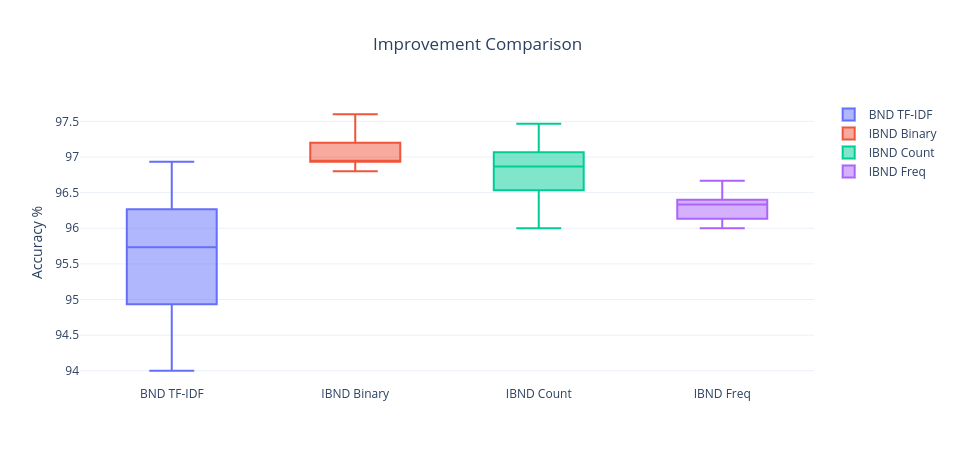
\includegraphics[width=1.5\textwidth]{imp}
  \caption{Standard Deviation of Results}
\end{figure}

\noindent
The baseline with new dataset using TF-IDF (BND TF-IDF) has an interquartile range of 1.36 while Improved baseline with new dataset using Binary (IBND Binary) has an interquartile range of 0.4 and higher max values. By switching the text representation methods and searching for the better find for this dataset, the model has gained around 1\% average improvement.

\section{Conclusion}
Overall, it’s worth testing different text representation methods as different contexts favour different methods. Which in this case the model gained around 1\% average improvement and 0.96 reduction in variance in evaluating the model. Further experimentation with changing text representation methods could explore including what type of words they are, i.e. nouns. 


\end{document}